% !TeX program = pdflatex
% =============================================================================
% Arbeitsblatt: Newtons Gesetze (nicht bewertet, Übungsmaterial für den Unterricht)
% Kantonsschule KFR – Physik, 4. Klasse, 1. HS, Mechanik
%
% Kopiert aus vorlagen/arbeitsblatt-vorlage.tex und um dieselben
% Farb-/Boxdefinitionen ergänzt wie kraefte-teil-1-arbeitsblatt.tex (gleicher
% Themencluster, direkt anschliessende Lektion). Templates sind
% selbstständig/nicht DRY, siehe CLAUDE.md.
%
% Scope (siehe lernziele.md, Abschnitt "Abgrenzung"): die drei Newtonschen
% Axiome (Trägheitsgesetz, Dynamisches Grundgesetz, Wechselwirkungsgesetz)
% als allgemeine Bewegungsgesetze, direkter Anschluss an Kräfte (Teil 1).
% Benannte Kraftarten MIT Formel (Gewichtskraft, Federkraft, Normalkraft,
% Reibungskraft) sind bewusst NICHT Teil dieser Einheit (folgen in Kräfte
% (Teil 2)); Gravitation/Himmelsmechanik und Scheinkräfte ebenfalls nicht.
% Deshalb wird im Aufzug-Beispiel die Gewichtskraft weiterhin direkt als
% Newton-Wert gegeben, nie über m*g berechnet.
%
% Stand: Lernziele, Einleitung, Theorie und Aufgaben fertig. LZ-Nummerierung
% entspricht der Dokumentreihenfolge und stimmt mit lernziele.md überein.
% =============================================================================
\documentclass[addpoints,11pt,a4paper]{exam}

\usepackage[T1]{fontenc}
\usepackage[utf8]{inputenc}
\usepackage[ngerman]{babel}
\usepackage{lmodern}
\usepackage[a4paper,margin=2.2cm,headheight=14pt]{geometry}
\usepackage{amsmath}
\usepackage{amssymb}
\usepackage{siunitx}
% Hausstil: zusammengesetzte Einheiten immer als echter Bruch (\frac), nicht
% als Schrägstrich inline oder \tfrac. Gilt global für jedes \si/\SI.
\sisetup{per-mode=fraction,fraction-command=\frac}
\usepackage{array,booktabs,tabularx,multirow}
\usepackage{enumitem}
\usepackage{graphicx}
\usepackage{xcolor}
\usepackage{colortbl}
\usepackage{tikz}
\usepackage{physics}
\usepackage{circuitikz}
\usepackage[most]{tcolorbox}
\usepackage{lastpage}

\usetikzlibrary{arrows.meta,calc,angles,quotes}

\setlength{\parindent}{0pt}
\setlength{\parskip}{0.45em}

% -----------------------------
% Farben (Hausfarbschema Physik KFR)
% -----------------------------
\definecolor{titleblue}{HTML}{183A6B}
\definecolor{accentblue}{HTML}{2E6F9E}
\definecolor{lightblue}{HTML}{EAF4FB}
\definecolor{verylightblue}{HTML}{F7FBFE}
\definecolor{lightgray}{HTML}{F4F6F8}
\definecolor{darkgray}{HTML}{4A4A4A}
\definecolor{accentorange}{HTML}{D9720C}
\definecolor{accentpurple}{HTML}{7B2D8E}
\definecolor{theorygreen}{HTML}{2E7D4F}
\definecolor{lighttheorygreen}{HTML}{EAF7EF}
\definecolor{groupteal}{HTML}{1B7F72}
\definecolor{lightgroupteal}{HTML}{E8F5F3}

% -----------------------------
% Spaltentypen
% -----------------------------
\newcolumntype{Y}{>{\centering\arraybackslash}X}
\newcolumntype{P}[1]{>{\raggedright\arraybackslash}p{#1}}

% -----------------------------
% Boxen
% -----------------------------
\newtcolorbox{titlebox}{
  enhanced,
  colback=titleblue,
  colframe=titleblue,
  boxrule=0pt,
  arc=3mm,
  left=3mm,right=3mm,top=3mm,bottom=3mm
}

\newlength{\aufgabenindent}
\settowidth{\aufgabenindent}{10.\hskip\labelsep}

\newtcolorbox{infobox}{
  enhanced,
  breakable,
  colback=lightblue,
  colframe=accentblue,
  boxrule=0.7pt,
  arc=2mm,
  left=5mm,right=5mm,top=2mm,bottom=2mm
}

\newtcolorbox{theoriebox}[1][Theorie]{
  enhanced,
  breakable,
  colback=lighttheorygreen,
  colframe=theorygreen,
  title={#1},
  fonttitle=\bfseries,
  boxrule=0.7pt,
  arc=2mm,
  left=5mm,right=5mm,top=2mm,bottom=2mm
}

\newtcolorbox{taskbox}[1][]{
  enhanced,
  breakable,
  colback=verylightblue,
  colframe=accentblue,
  title={#1},
  fonttitle=\bfseries,
  boxrule=0.7pt,
  arc=2mm,
  enlarge left by=-\aufgabenindent,
  width=\textwidth,
  left=5mm,right=5mm,top=2mm,bottom=2mm
}

\newtcolorbox{beispielbox}[1][Beispiel]{
  enhanced,
  breakable,
  colback=verylightblue,
  colframe=accentblue,
  title={#1},
  fonttitle=\bfseries,
  boxrule=0.7pt,
  arc=2mm,
  left=5mm,right=5mm,top=2mm,bottom=2mm
}

\newtcolorbox{groupbox}[1][Gruppenarbeit]{
  enhanced,
  breakable,
  colback=lightgroupteal,
  colframe=groupteal,
  title={#1},
  fonttitle=\bfseries,
  boxrule=0.7pt,
  arc=2mm,
  enlarge left by=-\aufgabenindent,
  width=\textwidth,
  left=5mm,right=5mm,top=2mm,bottom=2mm
}

\definecolor{lightorange}{HTML}{FCEEE0}
\newtcolorbox{hinweisbox}[1][Hinweis]{
  enhanced,
  breakable,
  colback=lightorange,
  colframe=accentorange,
  title={#1},
  fonttitle=\bfseries,
  boxrule=0.7pt,
  arc=2mm,
  left=5mm,right=5mm,top=2mm,bottom=2mm
}

% merksatzbox: eigene Farbe (Violett, wiederverwendet accentpurple), um die
% fundamentale Kernaussage (Formel und/oder Formulierung) jedes der drei
% Newtonschen Axiome innerhalb der jeweiligen (gruenen) theoriebox visuell
% klar hervorzuheben, deutlich staerker als blosses \textbf{\emph{...}}.
\definecolor{lightpurple}{HTML}{F3EAF7}
\newtcolorbox{merksatzbox}[1][Merksatz]{
  enhanced,
  breakable,
  colback=lightpurple,
  colframe=accentpurple,
  title={#1},
  fonttitle=\bfseries,
  boxrule=0.9pt,
  arc=2mm,
  left=5mm,right=5mm,top=2mm,bottom=2mm
}

\newtcolorbox{answerbox}{
  breakable,
  colback=white,
  colframe=gray!55,
  boxrule=0.5pt,
  arc=1.5mm,
  left=2mm,right=2mm,top=2mm,bottom=2mm
}

% --- Lösungen ein-/ausblenden -----------------------------------------------
\noprintanswers
% \printanswers

% --- Punkte bleiben intern, werden aber nicht gedruckt ----------------------
\pointformat{}

% --- Lösungsbox auf Deutsch, farblich abgesetzt -----------------------------
\renewcommand{\solutiontitle}{\noindent\color{titleblue}\textbf{Lösung:}\enspace}

% --- Kopf-/Fusszeile: Thema/Titel oben, Seitenzahl unten --------------------
\pagestyle{headandfoot}
\cfoot{\textcolor{darkgray}{Seite \thepage\ von \pageref{LastPage}}}

% --- Kopfzeile: Klasse / Datum / Thema / Titel ------------------------------
\newcommand{\Kopfzeile}[4]{%
  \begin{titlebox}
    {\color{white}\sffamily\bfseries\Large #4}
  \end{titlebox}
  \vspace{0.5em}
  \noindent\textbf{Klasse:}~#1 \hfill \textbf{Datum:}~#2 \hfill \textbf{Thema:}~#3
    \hfill \textbf{Lehrperson:}~Loris Keller
  \vspace{0.8em}
  \lhead{\textcolor{darkgray}{#3}}
  \rhead{\textcolor{darkgray}{#4}}
}

% --- Antwortraum: ca. 2.5 cm Platz pro Punkt, als umrandetes Feld -----------
\newlength{\antwortraumlen}
\newcommand{\Antwortraum}[1]{%
  \pgfmathsetlength{\antwortraumlen}{#1*2.5cm}%
  \begin{answerbox}
    \rule{0pt}{\antwortraumlen}%
  \end{answerbox}%
}

% Werte für Kopfzeile zentral setzen
\newcommand{\Klasse}{4a}
\newcommand{\Datum}{TT.MM.JJJJ}
\newcommand{\Thema}{Newtons Gesetze}
\newcommand{\ArbeitsblattTitel}{Arbeitsblatt: Newtons Gesetze}

\begin{document}

\Kopfzeile{\Klasse}{\Datum}{\Thema}{\ArbeitsblattTitel}

% --- Lernziele: aus lernziele.md (Backward-Design, Stufe 1) übernommen.
% LZ1..LZ9 entsprechen der Reihenfolge, in der die zugehörigen
% Theorieboxen/Übungen im Dokument erscheinen, identisch mit der
% Backward-Design-Reihenfolge, keine Umnummerierung nötig. --------------------
\begin{infobox}
\textbf{Lernziele}\\
Am Ende dieser Einheit kann ich \dots
\begin{itemize}[leftmargin=1.2cm,itemsep=0.25em]
  \item das 1. Newtonsche Gesetz (Trägheitsgesetz) in eigenen Worten formulieren und auf Beispiele in Ruhe oder mit konstanter Geschwindigkeit anwenden. (LZ1)
  \item erklären, warum ein Körper ohne resultierende Kraft seinen Bewegungszustand nicht ändert, auch wenn dieser einer Bewegung entspricht. (LZ2)
  \item das 2. Newtonsche Gesetz ($F=m\cdot a$) formulieren, die Einheit Newton aus den Grundeinheiten herleiten, und erklären, dass Kraft und Beschleunigung gleich gerichtet sind. (LZ3)
  \item das 2. Newtonsche Gesetz rechnerisch auf einfache Beispiele anwenden. (LZ4)
  \item an einem selbst durchgeführten Experiment den Zusammenhang zwischen Kraft, Masse und Beschleunigung überprüfen und auswerten. (LZ5)
  \item das 3. Newtonsche Gesetz (Wechselwirkungsgesetz) formulieren und an einem Beispiel mit zwei Körpern anwenden. (LZ6)
  \item das Wechselwirkungsgesetz vom Kräftegleichgewicht unterscheiden. (LZ7)
  \item erklären, dass auch passive Körper gemäss dem 3. Axiom eine Kraft ausüben. (LZ8)
  \item an einem zusammengesetzten Beispiel mehrere Axiome kombiniert anwenden. (LZ9)
\end{itemize}
\end{infobox}

% --- Einleitung: Voyager-1-Hook, direkt aus lernziele.md uebernommen. -----
\begin{beispielbox}[Einleitung: Voyager 1, ein (fast) kräftefreier Körper]
\begin{center}
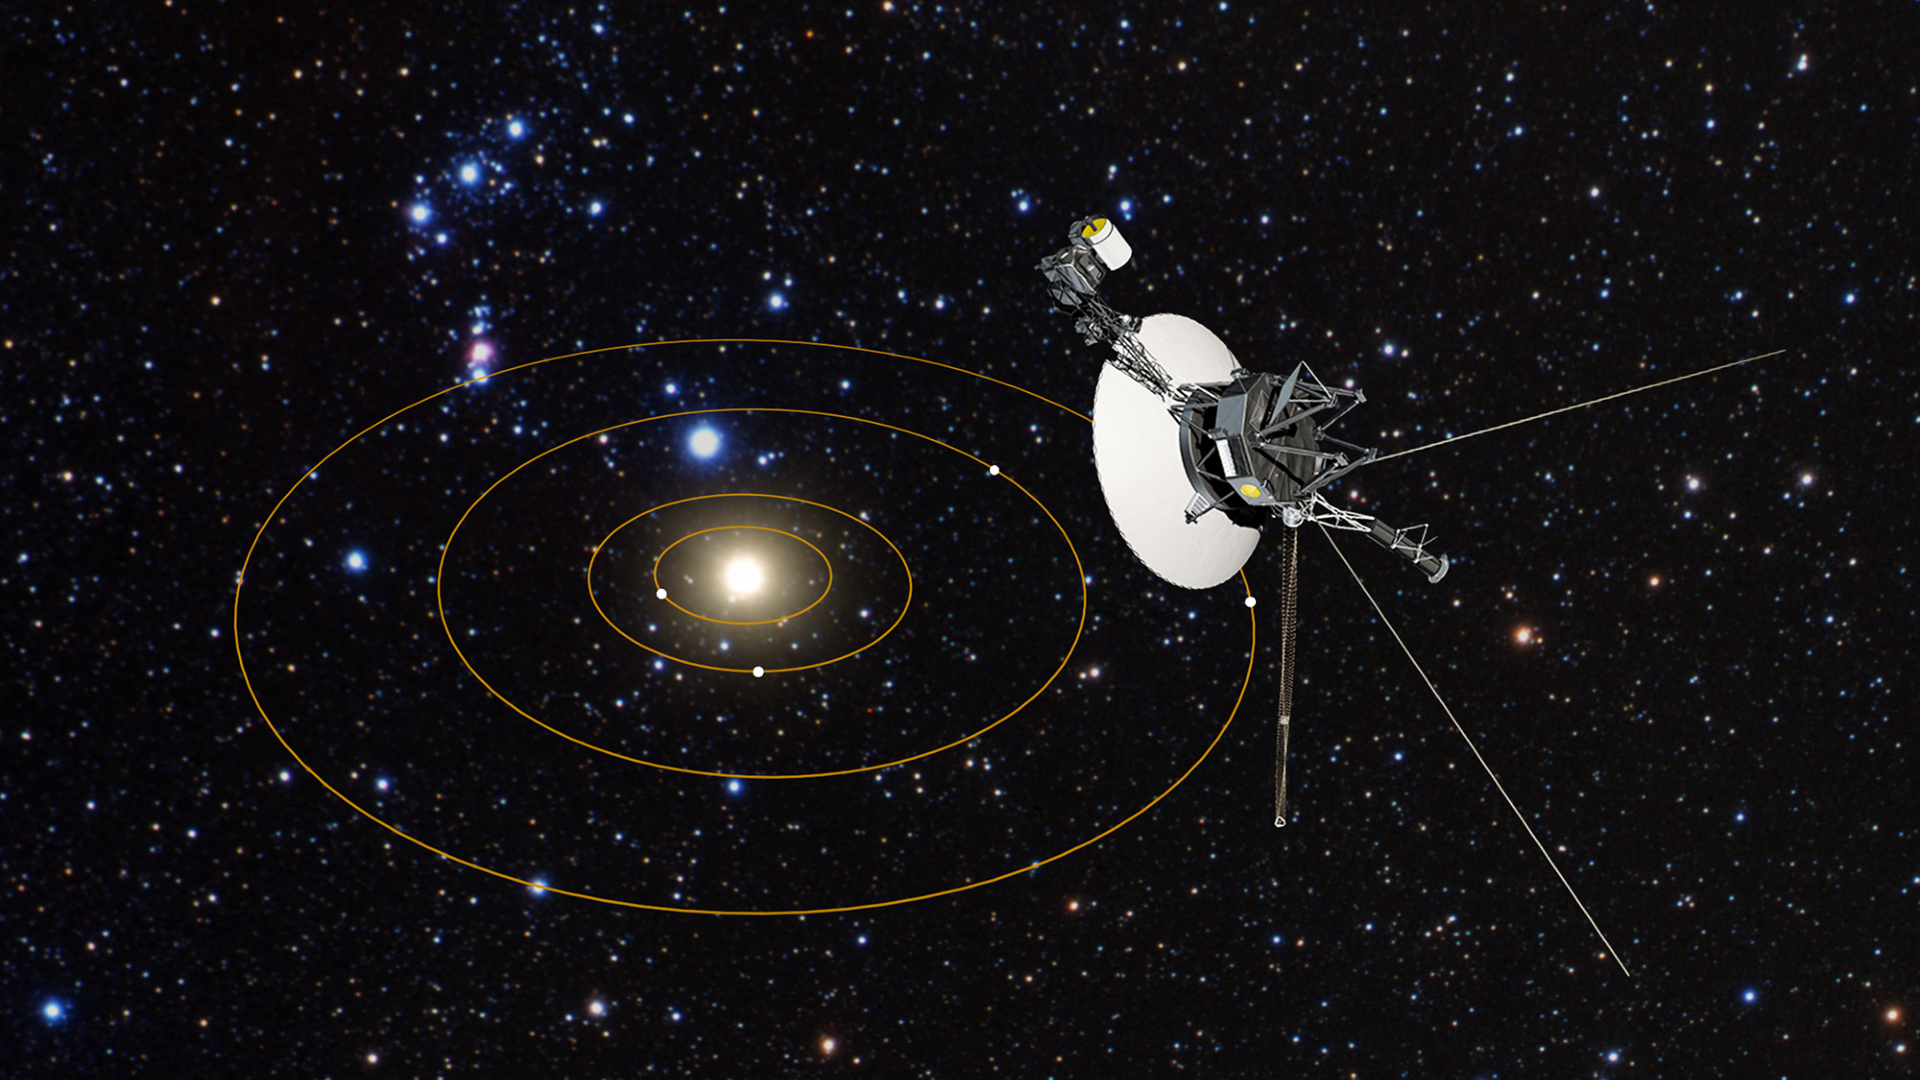
\includegraphics[width=0.6\linewidth]{Bilder/Voyager_1.jpg}
\end{center}
{\scriptsize Künstlerische Darstellung der Raumsonde Voyager 1, im
Hintergrund die Umlaufbahnen der äusseren Planeten unseres
Sonnensystems.}

Die Raumsonde Voyager 1 wurde 1977 von der NASA gestartet. Seit 2012 hat
sie das Sonnensystem verlassen und bewegt sich seither mit konstant rund
\SI{61000}{\kilo\meter\per\hour} geradlinig weiter durch den
interstellaren Raum, ganz ohne Antrieb. Kein Treibstoff, kein Motor, kaum
messbare Kräfte wirken noch auf sie, trotzdem wird sie weder langsamer
noch ändert sie ihre Richtung.

Voyager 1 ist einer der wenigen realen Fälle eines fast vollständig
kräftefreien Körpers. Auf der Erde begegnet man diesem Zustand kaum,
weil hier praktisch immer Reibung oder Luftwiderstand wirkt, aber genau
dieser Grenzfall, ein Körper ganz ohne resultierende Kraft, steht im
Zentrum des Gesetzes, das du in diesem Kapitel kennenlernst.
\end{beispielbox}

% --- Tischdecken-Trick als POE, direkt im Anschluss (nicht als zweiter
% Hook), wie in lernziele.md vorgeschlagen. Adressiert Lernschwierigkeit 1
% durch kognitiven Konflikt, bevor die Theoriebox formalisiert. ------------
\begin{groupbox}[Predict-Observe-Explain: Der Tischdeckentrick]
Auf einem Tisch steht Geschirr (Teller, Gläser) auf einer Tischdecke.
Jemand zieht die Tischdecke ruckartig und mit einem einzigen schnellen
Zug waagrecht weg.

\begin{parts}
  \part[2] \textbf{Predict:} Was, denkst du, passiert mit dem Geschirr?
  Notiere deine Vorhersage und eine kurze Begründung, bevor ihr es
  testet oder ein Video seht.
  \Antwortraum{2}

  \part[1] \textbf{Observe:} Was ist tatsächlich passiert?
  \Antwortraum{1}

  \part[3] \textbf{Explain:} Stimmt deine Vorhersage mit der Beobachtung
  überein? Warum bleibt das Geschirr (fast) an Ort und Stelle, obwohl die
  Tischdecke plötzlich weg ist?
  \Antwortraum{3}
\end{parts}

\begin{center}
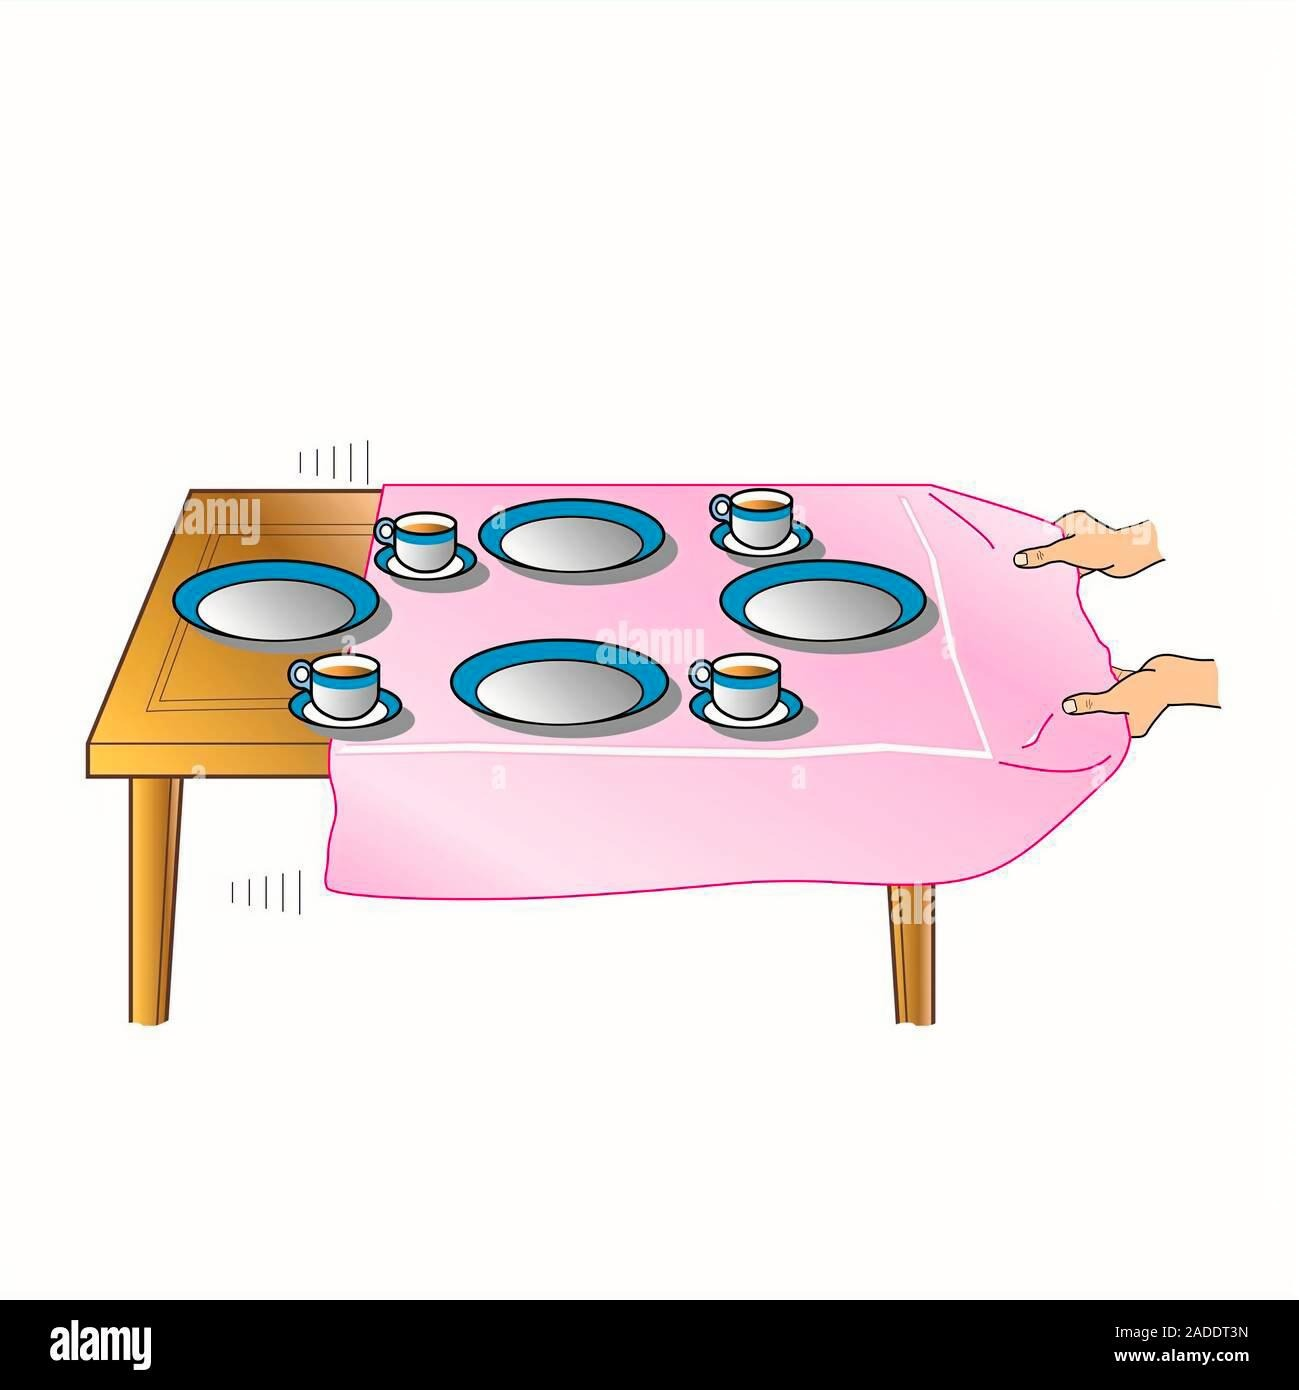
\includegraphics[width=0.55\linewidth]{Bilder/Tischdeckentrick.jpg}
\end{center}
{\scriptsize So sieht der Tischdeckentrick aus: Die Tischdecke wird
ruckartig weggezogen, das Geschirr bleibt (fast) an Ort und Stelle
stehen. Schau dir das Bild erst \textbf{nach} deiner Vorhersage in
Teilaufgabe a) an.}
\end{groupbox}

\begin{taskbox}[Plenumsdiskussion]
Vergleicht in der Klasse eure Erklärungen zum Tischdeckentrick mit dem
Voyager-1-Beispiel aus der Einleitung. Was haben ein ruhendes Geschirr
und eine mit konstanter Geschwindigkeit fliegende Raumsonde gemeinsam?
Sammelt gemeinsam eine erste, vorläufige Formulierung eines Gesetzes,
bevor ihr die Theoriebox unten lest.
\end{taskbox}

\begin{theoriebox}[Das 1. Newtonsche Gesetz: Trägheitsgesetz]
\begin{merksatzbox}
Ein Körper bleibt in Ruhe oder bewegt sich mit konstanter Geschwindigkeit
geradlinig weiter, solange keine resultierende Kraft auf ihn wirkt
($F_{\text{res}}=\SI{0}{\newton}$).
\end{merksatzbox}

Diese Eigenschaft, dem eigenen Bewegungszustand \glqq treu zu bleiben\grqq{}
und sich einer Änderung zu widersetzen, nennt man \textbf{\emph{Trägheit}}.
Das 1. Newtonsche Gesetz wird deshalb auch \textbf{\emph{Trägheitsgesetz}}
genannt.

\textbf{Wichtig:} \glqq Ruhe\grqq{} ist dabei nur ein \textbf{\emph{Spezialfall}}
von \glqq konstanter Geschwindigkeit\grqq{}, nämlich der Fall
$v=\SI{0}{\meter\per\second}$. Aus Sicht des Trägheitsgesetzes sind Ruhe
und gleichförmige geradlinige Bewegung völlig gleichwertig: Beide
Zustände bleiben ohne resultierende Kraft von selbst erhalten. Das
Geschirr beim Tischdeckentrick bleibt in Ruhe, Voyager~1 bleibt in
gleichförmiger Bewegung, beide aus demselben Grund.

Dieses Gesetz kennst du in Teilen bereits aus Kräfte (Teil 1): Dort hast
du gelernt, dass Kräftegleichgewicht ($F_{\text{res}}=\SI{0}{\newton}$)
Ruhe bedeuten kann. Das 1. Newtonsche Gesetz erweitert das jetzt: Ohne
resultierende Kraft bleibt ein Körper entweder in Ruhe \textbf{oder} in
gleichförmiger Bewegung, je nachdem, welchen Bewegungszustand er vorher
hatte.
\end{theoriebox}

\begin{hinweisbox}[Hinweis: \glqq Bewegung braucht immer eine Kraft\grqq{} stimmt nicht]
Im Alltag scheint es so, als würde jede Bewegung irgendwann von selbst
aufhören, wenn man nicht weiter antreibt (ein rollender Ball, ein
ausrollendes Fahrrad). Das liegt aber \textbf{nicht} daran, dass
Bewegung eine \glqq Kraft verbraucht\grqq{}, die \glqq aufgebraucht\grqq{}
wird, sondern daran, dass auf der Erde fast immer eine bremsende Kraft
wirkt (Reibung, Luftwiderstand). Ohne diese bremsenden Kräfte, wie bei
Voyager~1 im Weltraum, bleibt die Geschwindigkeit konstant, für immer.
Ein bewegter Körper \glqq enthält\grqq{} also keine Kraft, die
irgendwann aufgebraucht wäre.
\end{hinweisbox}

\begin{questions}
\begin{taskbox}[Übung: Trägheitsgesetz anwenden]
\question[6] Entscheide für jede Situation: Wirkt eine resultierende
Kraft auf den Körper, oder nicht? Begründe jeweils mit dem
Trägheitsgesetz.

\begin{parts}
  \part[2] Ein Eishockeypuck gleitet über eine (näherungsweise
  reibungsfreie) Eisfläche mit konstanter Geschwindigkeit geradeaus.
  \Antwortraum{2}
  \begin{solution}
  Keine resultierende Kraft ($F_{\text{res}}=\SI{0}{\newton}$): Die
  Geschwindigkeit ist konstant und geradlinig, genau das erwartet das
  Trägheitsgesetz ohne Krafteinwirkung.
  \end{solution}

  \part[2] Ein Buch liegt ruhig auf einem Tisch.
  \Antwortraum{2}
  \begin{solution}
  Keine resultierende Kraft: Das Buch ist in Ruhe (ein Spezialfall
  konstanter Geschwindigkeit, $v=\SI{0}{\meter\per\second}$) und bleibt
  es, solange sich nichts ändert. (Einzelne Kräfte wie Gewichtskraft und
  Normalkraft wirken zwar, heben sich aber auf, siehe Kräfte Teil 1.)
  \end{solution}

  \part[2] Ein Fahrrad rollt aus und wird dabei langsamer.
  \Antwortraum{2}
  \begin{solution}
  Hier wirkt eine resultierende Kraft (Reibung, Luftwiderstand): Die
  Geschwindigkeit ändert sich (wird kleiner), das widerspricht dem
  Trägheitsgesetz nur scheinbar, weil eben doch eine bremsende Kraft
  wirkt und der Fall damit nicht kräftefrei ist.
  \end{solution}
\end{parts}
\end{taskbox}
\end{questions}

\begin{theoriebox}[Das 2. Newtonsche Gesetz: Dynamisches Grundgesetz]
Was passiert, wenn eben doch eine resultierende Kraft wirkt? Das 2.
Newtonsche Gesetz beantwortet das:

\begin{merksatzbox}
\[
  F_{\text{res}} = m\cdot a, \qquad \text{bzw. umgestellt} \qquad
  a = \frac{F_{\text{res}}}{m}.
\]
\end{merksatzbox}

\textbf{Zwei Zusammenhänge stecken in dieser Formel:}
\begin{itemize}[leftmargin=1.2cm,itemsep=0.25em]
  \item Je \textbf{\emph{grösser}} die resultierende Kraft, desto
  \textbf{\emph{grösser}} die Beschleunigung (bei gleicher Masse):
  $F_{\text{res}}$ und $a$ sind proportional.
  \item Je \textbf{\emph{grösser}} die Masse, desto \textbf{\emph{kleiner}}
  die Beschleunigung (bei gleicher Kraft): Ein schwererer Körper lässt
  sich schwerer beschleunigen, nicht leichter. $m$ und $a$ sind
  \textbf{\emph{umgekehrt proportional}} (bei fester Kraft).
\end{itemize}

Ausserdem gilt: Die Beschleunigung $a$ zeigt immer in \textbf{\emph{dieselbe
Richtung}} wie die resultierende Kraft $F_{\text{res}}$.

\textbf{Die Einheit Newton hergeleitet:} In Kräfte (Teil 1) hast du
Newton nur als eigene, vorgegebene Einheit kennengelernt. Jetzt kannst du
sie aus den Grundeinheiten herleiten, indem du die Einheiten von
$F=m\cdot a$ einsetzt.

\textbf{Schritt 1:} Einheiten von $m$ und $a$ einsetzen:
\[
  [F] = [m]\cdot[a] = \si{\kilo\gram}\cdot\si{\meter\per\second\squared}.
\]
\textbf{Schritt 2:} Als Definition der Einheit Newton festhalten:
\[
  \boxed{\SI{1}{\newton} = \SI{1}{\kilo\gram\meter\per\second\squared}}.
\]
\end{theoriebox}

\begin{hinweisbox}[Hinweis: keine \glqq Kraftformel unter vielen\grqq{}]
$F_{\text{res}}=m\cdot a$ ist keine Formel unter vielen, sondern die
\textbf{\emph{grundlegende Beziehung}} zwischen Kraft, Masse und
Beschleunigung, gültig für jede resultierende Kraft und jeden Körper.
Wirken mehrere einzelne Kräfte gleichzeitig (wie in Kräfte Teil 1
addiert), setzt du für $F_{\text{res}}$ immer zuerst deren
\textbf{\emph{Summe}} ein, nie eine einzelne der beteiligten Kräfte
allein.
\end{hinweisbox}

\begin{questions}
\begin{taskbox}[Clicker-ConcepTest: Kräftewettstreit]
\question[3] Ein Auto ($m=\SI{1000}{\kilo\gram}$) wird vom Motor mit
$F_{\text{Motor}}=\SI{2000}{\newton}$ nach vorne angetrieben. Gleichzeitig
wirkt eine Reibungskraft von $F_R=\SI{500}{\newton}$ entgegen der
Fahrtrichtung.

\begin{parts}
  \part[3] Wie berechnest du die Beschleunigung des Autos richtig?
  Kreuze an und begründe.
  \begin{itemize}[leftmargin=1.2cm,itemsep=0.15em]
    \item[$\square$] A: $a = F_{\text{Motor}}/m$, die Reibungskraft
    zählt nicht mit, weil sie nur \glqq bremst\grqq{}, aber nicht
    \glqq antreibt\grqq{}.
    \item[$\square$] B: $a = (F_{\text{Motor}}-F_R)/m$, weil für das 2.
    Newtonsche Gesetz immer die \textbf{resultierende} Kraft eingesetzt
    werden muss.
    \item[$\square$] C: $a=\SI{0}{\meter\per\second\squared}$, weil sich
    zwei Kräfte gegenseitig \glqq blockieren\grqq{}, sobald beide
    gleichzeitig wirken.
  \end{itemize}
  \Antwortraum{2}
  \begin{solution}
  Richtig ist \textbf{B}. $F_{\text{res}}=F_{\text{Motor}}-F_R=
  \SI{2000}{\newton}-\SI{500}{\newton}=\SI{1500}{\newton}$, also
  $a=F_{\text{res}}/m=\SI{1500}{\newton}/\SI{1000}{\kilo\gram}=
  \SI{1.5}{\meter\per\second\squared}$. Aussage A ignoriert, dass $F=ma$
  die resultierende Kraft verlangt, nicht nur die \glqq antreibende\grqq{}
  Einzelkraft. Aussage C verwechselt \glqq zwei Kräfte wirken
  gleichzeitig\grqq{} mit \glqq die Kräfte heben sich zwingend auf\grqq{},
  das stimmt nur, wenn sie exakt gleich gross sind (hier nicht der Fall).
  \end{solution}
\end{parts}
\end{taskbox}
\end{questions}

% --- Luftkissenbahn-Experiment (LZ4-5), POE-Prinzip, Gruppenarbeit, wie in
% lernziele.md vorgeschlagen (phyphox-App, "Linear acceleration on an air
% track"). Bewusst ohne erfundene Messwerte, da echtes Experiment. ---------
\begin{groupbox}[Experiment: Kraft, Masse und Beschleunigung auf der Luftkissenbahn]
Auf der Luftkissenbahn gleitet ein Wagen (näherungsweise) reibungsfrei
auf einem Luftpolster. Über eine Schnur und eine Umlenkrolle zieht ein
Hängegewicht den Wagen mit einer bekannten Kraft $F$ an. Mit der
phyphox-App (Sensor \glqq Beschleunigung ohne g\grqq{} bzw. \glqq Linear
Acceleration\grqq{}, Smartphone auf dem Wagen befestigt) misst ihr die
Beschleunigung $a$ des Wagens.

\begin{parts}
  \part[3] \textbf{Predict:} Was passiert mit $a$, wenn ihr die
  ziehende Kraft $F$ verdoppelt (z.\,B. durch ein zweites
  Hängegewicht), bei gleichbleibender Wagenmasse $m$? Was passiert mit
  $a$, wenn ihr stattdessen die Wagenmasse $m$ verdoppelt
  (Zusatzgewicht auf den Wagen), bei gleichbleibender Kraft $F$? Notiert
  eure Vorhersagen, bevor ihr testet.
  \Antwortraum{3}

  \part[5] \textbf{Observe:} Führt mindestens vier Messungen durch:
  zwei mit unterschiedlicher Kraft $F$ bei gleicher Masse $m$, zwei mit
  unterschiedlicher Masse $m$ bei gleicher Kraft $F$. Tragt eure
  Messwerte in die Tabelle ein.
  \begin{center}
  \begin{tabular}{@{}lllll@{}}
  \toprule
  Messung & $F$ in $\si{\newton}$ & $m$ in $\si{\kilo\gram}$ & $a$ in $\si{\meter\per\second\squared}$ & $F/a$ in $\si{\kilo\gram}$ \\
  \midrule
  1 & & & & \\[0.8em]
  2 & & & & \\[0.8em]
  3 & & & & \\[0.8em]
  4 & & & & \\[0.8em]
  \bottomrule
  \end{tabular}
  \end{center}

  \part[4] \textbf{Explain:} Berechnet für jede Messung das Verhältnis
  $F/a$ und vergleicht es mit der jeweiligen Masse $m$ aus der Tabelle.
  Was fällt auf? Stimmen eure Vorhersagen aus a) mit euren Beobachtungen
  überein? Formuliert euer Ergebnis als Satz.
  \Antwortraum{4}
  \begin{solution}
  Bei korrekter Durchführung sollte $F/a \approx m$ gelten (im Rahmen
  der Messgenauigkeit), da $F=m\cdot a$ nach $m=F/a$ umgestellt genau
  das vorhersagt. Verdoppelt man $F$ bei gleicher Masse, sollte sich
  $a$ ebenfalls verdoppeln; verdoppelt man $m$ bei gleicher Kraft,
  sollte sich $a$ halbieren. Individuelle Messwerte und Formulierungen
  von der Lehrperson zu kontrollieren.
  \end{solution}
\end{parts}
\end{groupbox}

\begin{questions}
\begin{taskbox}[Produktives Üben: Das 2. Newtonsche Gesetz berechnen]
\question[4] Ein E-Bike mit Masse $m=\SI{25}{\kilo\gram}$ wird mit einer
resultierenden Kraft von $F_{\text{res}}=\SI{50}{\newton}$ beschleunigt.

\begin{parts}
  \part[2] Berechne die Beschleunigung $a$.
  \Antwortraum{2}
  \begin{solution}
  \[
    a = \frac{F_{\text{res}}}{m} = \frac{\SI{50}{\newton}}{\SI{25}{\kilo\gram}} = \SI{2}{\meter\per\second\squared}.
  \]
  \end{solution}

  \part[2] Zeige durch Einsetzen der Einheiten (nicht der Zahlenwerte),
  dass bei dieser Rechnung tatsächlich $\si{\meter\per\second\squared}$
  herauskommt. In welche Richtung zeigt $a$, wenn $F_{\text{res}}$ in
  Fahrtrichtung nach vorne zeigt?
  \Antwortraum{2}
  \begin{solution}
  \[
    [a] = \frac{[F_{\text{res}}]}{[m]} = \frac{\si{\newton}}{\si{\kilo\gram}} = \frac{\si{\kilo\gram\meter\per\second\squared}}{\si{\kilo\gram}} = \si{\meter\per\second\squared}.
  \]
  Die Beschleunigung $a$ zeigt in dieselbe Richtung wie $F_{\text{res}}$,
  hier also ebenfalls nach vorne.
  \end{solution}
\end{parts}

\question[2] Ein Einkaufswagen mit Masse $m=\SI{15}{\kilo\gram}$ soll mit
$a=\SI{0.8}{\meter\per\second\squared}$ beschleunigt werden.

\begin{parts}
  \part[2] Welche resultierende Kraft ist dafür nötig?
  \Antwortraum{2}
  \begin{solution}
  \[
    F_{\text{res}} = m\cdot a = \SI{15}{\kilo\gram}\cdot\SI{0.8}{\meter\per\second\squared} = \SI{12}{\newton}.
  \]
  \end{solution}
\end{parts}

\question[5] Ein Auto wird mit $F_{\text{res}}=\SI{3000}{\newton}$
beschleunigt und erreicht dabei $a=\SI{2}{\meter\per\second\squared}$.

\begin{parts}
  \part[3] Berechne die Masse des Autos.
  \Antwortraum{3}
  \begin{solution}
  \[
    m = \frac{F_{\text{res}}}{a} = \frac{\SI{3000}{\newton}}{\SI{2}{\meter\per\second\squared}} = \SI{1500}{\kilo\gram}.
  \]
  \end{solution}

  \part[2] Vergleiche dein Vorgehen hier mit dem
  Luftkissenbahn-Experiment weiter oben: Wie hättest du dort die Masse
  des Wagens allein aus den gemessenen Werten $F$ und $a$ bestimmen
  können, ohne den Wagen zu wägen?
  \Antwortraum{2}
  \begin{solution}
  Genau gleich wie hier, mit $m=F/a$: Auch beim Luftkissenbahn-Experiment
  hätte das Verhältnis $F/a$ aus jeder einzelnen Messung direkt die
  (unbekannte) Masse des Wagens ergeben müssen, ganz ohne Waage.
  \end{solution}
\end{parts}
\end{taskbox}
\end{questions}

\begin{theoriebox}[Das 3. Newtonsche Gesetz: Wechselwirkungsgesetz]
\begin{merksatzbox}
Übt ein Körper A eine Kraft (Aktionskraft) auf einen Körper B aus, so
übt B gleichzeitig eine gleich grosse, aber entgegengesetzt gerichtete
Kraft (Reaktionskraft) auf A aus.
\[
  F_{A\to B} = -F_{B\to A}.
\]
\end{merksatzbox}

Drei Eigenschaften eines solchen \textbf{\emph{Wechselwirkungspaars}}
(auch als Aktio und Reaktio bezeichnet) sind besonders wichtig:
\begin{itemize}[leftmargin=1.2cm,itemsep=0.2em]
  \item Beide Kräfte wirken \textbf{\emph{gleichzeitig}}, keine der
  beiden \glqq verursacht\grqq{} die andere zeitlich verzögert.
  \item Beide Kräfte sind vom \textbf{\emph{gleichen Typ}} (z.\,B. beide
  Kontaktkräfte oder beide Gravitationskräfte).
  \item Beide Kräfte wirken auf \textbf{\emph{zwei verschiedene
  Körper}}, niemals auf denselben Körper. Genau das unterscheidet sie
  von einem Kräftegleichgewicht, siehe Hinweisbox weiter unten.
\end{itemize}
\end{theoriebox}

\begin{groupbox}[Think-Pair-Share: Zwei Eisläuferinnen stossen sich ab]
Zwei Eisläuferinnen stehen sich auf einer reibungsfreien Eisfläche
gegenüber und stossen sich gleichzeitig voneinander ab. Person A hat
Masse $m_A=\SI{60}{\kilo\gram}$, Person B hat Masse
$m_B=\SI{90}{\kilo\gram}$. Nach dem 3. Newtonschen Gesetz ist die Kraft,
mit der A auf B drückt, exakt gleich gross wie die Kraft, mit der B auf
A drückt: $F=\SI{180}{\newton}$ (für beide gleich, nur entgegengesetzt
gerichtet).

\begin{parts}
  \part[2] \textbf{Think:} Wer bewegt sich nach dem Abstossen schneller
  weg, A oder B, oder gleich schnell? Notiere zuerst deine eigene
  Vermutung und Begründung, bevor du rechnest.
  \Antwortraum{2}

  \part[4] \textbf{Pair:} Berechnet zu zweit die Beschleunigung von A
  und von B während des Abstossens, mit dem 2. Newtonschen Gesetz.
  Vergleicht das Ergebnis mit eurer Vermutung aus a).
  \Antwortraum{4}
  \begin{solution}
  \[
    a_A = \frac{F}{m_A} = \frac{\SI{180}{\newton}}{\SI{60}{\kilo\gram}} = \SI{3}{\meter\per\second\squared},
    \qquad
    a_B = \frac{F}{m_B} = \frac{\SI{180}{\newton}}{\SI{90}{\kilo\gram}} = \SI{2}{\meter\per\second\squared}.
  \]
  Person A (die leichtere) wird stärker beschleunigt als Person B (die
  schwerere), obwohl beide exakt dieselbe Kraft erfahren (3. Axiom): Die
  Kraft ist gleich, aber wegen der unterschiedlichen Masse ist die
  Beschleunigung unterschiedlich (2. Axiom).
  \end{solution}

  \part[2] \textbf{Share:} Erklärt in eigenen Worten, warum \glqq gleich
  grosse Kraft für beide\grqq{} nicht \glqq gleich grosse Beschleunigung
  für beide\grqq{} bedeutet.
  \Antwortraum{2}
  \begin{solution}
  Das 3. Axiom garantiert nur, dass die \emph{Kräfte} gleich gross sind,
  nicht die \emph{Beschleunigungen}: Die Beschleunigung hängt zusätzlich
  von der Masse ab ($a=F/m$), und die beiden Personen haben
  unterschiedliche Massen.
  \end{solution}
\end{parts}
\end{groupbox}

% --- Whiteboarding mit getrennten Körperskizzen (LZ6-8), wie in
% lernziele.md vorgeschlagen (Schecker & Wilhelm: ein Körper pro Skizze). --
\begin{groupbox}[Whiteboarding: Zwei getrennte Kräftebilder]
Zeichnet auf einem Whiteboard oder A3-Blatt \textbf{zwei separate}
Kräftebilder für die Eisläuferinnen aus der vorherigen Aufgabe, während
sie sich gerade abstossen: eines für Person A, eines für Person B, klar
räumlich getrennt.

\begin{parts}
  \part[3] Zeichnet in \textbf{jedes} der beiden Kräftebilder alle
  Kräfte ein, die auf die jeweilige Person wirken: die Gewichtskraft
  (nach unten), die Normalkraft des Eises (nach oben) und die
  Abstosskraft der jeweils anderen Person (horizontal, $\SI{180}{\newton}$).
  \Antwortraum{3}

  \part[3] Markiert farbig, welche zwei Kräfte in euren beiden
  Zeichnungen ein \textbf{Wechselwirkungspaar} (3. Axiom) bilden.
  Erklärt, warum diese beiden Kräfte zwingend in \textbf{zwei
  verschiedenen} Kräftebildern stehen müssen und nicht in einem einzigen.
  \Antwortraum{3}
  \begin{solution}
  Die horizontalen Abstosskräfte (A auf B und B auf A) bilden das
  Wechselwirkungspaar: gleich gross, entgegengesetzt gerichtet, aber sie
  wirken auf zwei verschiedene Körper (A bzw. B), deshalb gehören sie in
  zwei getrennte Kräftebilder. Die vertikalen Kräfte (Gewichtskraft und
  Normalkraft) innerhalb je eines Kräftebilds bilden dagegen \emph{kein}
  Wechselwirkungspaar, sondern ein Kräftegleichgewicht am selben Körper,
  siehe Hinweisbox unten.
  \end{solution}
\end{parts}
\end{groupbox}

\begin{hinweisbox}[Hinweis: Wechselwirkungspaar oder Kräftegleichgewicht?]
Diese beiden Situationen sehen sich zum Verwechseln ähnlich, sind aber
grundverschieden. Am Beispiel eines Buchs, das ruhig auf einem Tisch
liegt:

\begin{center}
\begin{tikzpicture}[scale=1.4]
  % Panel 1: Kraeftegleichgewicht am Buch (ein Koerper)
  \draw[thick,fill=lightgray] (-0.7,0) rectangle (0.7,0.4);
  \node at (0,0.2) {\scriptsize Buch};
  \draw[->,thick,titleblue] (0,0) -- (0,-1.1) node[below] {\scriptsize $F_G$};
  \draw[->,thick,accentorange] (0,0.4) -- (0,1.5) node[above] {\scriptsize $F_N$};
  \node[align=center] at (0,-2.0) {\scriptsize Kräftegleichgewicht\\\scriptsize (ein Körper: Buch)};

  % Panel 2: Wechselwirkungspaar (zwei Koerper)
  \begin{scope}[xshift=6cm]
    \draw[thick,fill=lightgray] (-0.7,0.6) rectangle (0.7,1.0);
    \node at (0,0.8) {\scriptsize Buch};
    \draw[thick,fill=gray!30] (-1.1,-0.5) rectangle (1.1,0);
    \node at (0,-0.25) {\scriptsize Tisch};
    \draw[->,thick,accentpurple] (0.3,0.6) -- (0.3,0.05) node[midway,right] {\scriptsize $F_N'$};
    \draw[->,thick,accentorange] (-0.3,0) -- (-0.3,0.55) node[midway,left] {\scriptsize $F_N$};
    \node[align=center] at (0,-1.1) {\scriptsize Wechselwirkungspaar\\\scriptsize (zwei Körper: Buch \& Tisch)};
  \end{scope}
\end{tikzpicture}
\end{center}

\textbf{Links, Kräftegleichgewicht:} Auf das Buch (\textbf{ein einziger}
Körper) wirken zwei Kräfte, die Gewichtskraft $F_G$ (Erde zieht Buch
nach unten) und die Normalkraft $F_N$ (Tisch drückt Buch nach oben).
Diese beiden sind zufällig gleich gross, \textbf{weil} das Buch in Ruhe
ist ($F_{\text{res}}=\SI{0}{\newton}$, 1. Axiom), nicht wegen des 3.
Axioms.

\textbf{Rechts, Wechselwirkungspaar:} Der Tisch drückt mit der Kraft
$F_N$ nach oben auf das Buch, das Buch drückt mit der gleich grossen
Kraft $F_N'$ nach unten auf den Tisch. Diese beiden Kräfte wirken auf
\textbf{zwei verschiedene} Körper (Buch und Tisch) und sind nach dem 3.
Axiom \textbf{immer} gleich gross, unabhängig davon, ob sich irgendetwas
bewegt oder nicht.

\textbf{Merke:} Kräftegleichgewicht $\to$ mehrere Kräfte an
\textbf{einem} Körper, zufällig im Gleichgewicht. Wechselwirkungspaar
$\to$ je eine Kraft an \textbf{zwei verschiedenen} Körpern, immer gleich
gross.
\end{hinweisbox}

\begin{questions}
\begin{taskbox}[Clicker-ConcepTest: Übt jeder Körper eine Kraft aus?]
\question[4] Ein LKW und ein PKW stossen frontal zusammen.

\begin{parts}
  \part[2] Welche Aussage ist richtig? Kreuze an.
  \begin{itemize}[leftmargin=1.2cm,itemsep=0.15em]
    \item[$\square$] A: Der LKW übt eine grössere Kraft auf den PKW aus
    als der PKW auf den LKW, weil der LKW schwerer ist.
    \item[$\square$] B: Beide Fahrzeuge üben exakt die gleiche Kraft
    aufeinander aus, auch wenn ihre Beschleunigungen wegen der
    unterschiedlichen Massen verschieden gross sind.
    \item[$\square$] C: Nur der LKW übt eine Kraft aus, der PKW leistet
    nur passiven Widerstand.
  \end{itemize}
  \Antwortraum{2}
  \begin{solution}
  Richtig ist \textbf{B}, nach dem 3. Axiom. Aussage A verwechselt Masse
  mit Kraft: \glqq schwerer\grqq{} bedeutet nicht \glqq übt automatisch
  mehr Kraft aus\grqq{}. Aussage C nimmt an, nur \glqq aktive\grqq{}
  Körper könnten Kräfte ausüben, auch der PKW, obwohl er die
  \glqq schwächere\grqq{} Seite ist, übt zwingend eine gleich grosse
  Gegenkraft aus. (Die \textbf{Beschleunigungen} unterscheiden sich
  trotzdem deutlich, weil der PKW die kleinere Masse hat, siehe 2.
  Axiom, wie bei den Eisläuferinnen oben.)
  \end{solution}

  \part[2] Ein Tisch \glqq leistet nur Widerstand\grqq{}, wenn ein Buch
  auf ihm liegt, er übt selbst aber keine Kraft aus, sagt ein Mitschüler.
  Stimmt das? Begründe mit dem 3. Axiom.
  \Antwortraum{2}
  \begin{solution}
  Nein, das stimmt nicht. Auch ein passiver, unbeweglicher Körper wie
  ein Tisch übt eine echte Kraft aus (die Normalkraft $F_N$ auf das
  Buch), sonst könnte das Buch nicht in Ruhe bleiben. Nach dem 3. Axiom
  übt das Buch gleichzeitig eine gleich grosse Gegenkraft auf den Tisch
  aus.
  \end{solution}
\end{parts}
\end{taskbox}
\end{questions}

% --- Aufzug-Szenario (LZ9), kombiniert 2. und 3. Axiom, wie in
% lernziele.md vorgeschlagen. Gewichtskraft bewusst direkt gegeben (nicht
% ueber m*g berechnet), Masse separat gegeben, siehe Scope-Hinweis oben. ---
\begin{questions}
\begin{taskbox}[Produktives Üben: Der Aufzug (2. und 3. Axiom kombiniert)]
\question[9] Eine Person mit Masse $m=\SI{70}{\kilo\gram}$ und
Gewichtskraft $F_G=\SI{700}{\newton}$ steht auf einer Waage in einem
Aufzug. Die Waage zeigt die Kraft an, mit der die Person auf sie drückt.

\begin{parts}
  \part[2] Der Aufzug steht still. Welche Kraft zeigt die Waage an?
  Begründe mit dem 1. Axiom.
  \Antwortraum{2}
  \begin{solution}
  Der Aufzug steht still, also ist $F_{\text{res}}=\SI{0}{\newton}$ (1.
  Axiom). Die Normalkraft der Waage muss die Gewichtskraft also genau
  ausgleichen: $F_N=F_G=\SI{700}{\newton}$. Nach dem 3. Axiom zeigt die
  Waage exakt diese Kraft an.
  \end{solution}

  \part[4] Der Aufzug beschleunigt mit $a=\SI{2}{\meter\per\second\squared}$
  nach oben. Berechne mit dem 2. Axiom die Normalkraft $F_N$, die die
  Waage jetzt auf die Person ausübt (nach oben positiv:
  $F_N-F_G=m\cdot a$).
  \Antwortraum{4}
  \begin{solution}
  \[
    F_N - F_G = m\cdot a
    \quad\Longrightarrow\quad
    F_N = F_G + m\cdot a = \SI{700}{\newton} + \SI{70}{\kilo\gram}\cdot\SI{2}{\meter\per\second\squared}.
  \]
  \[
    F_N = \SI{700}{\newton} + \SI{140}{\newton} = \SI{840}{\newton}.
  \]
  Die Waage zeigt jetzt eine grössere Kraft an als im Stillstand: Man
  fühlt sich beim Beschleunigen nach oben \glqq schwerer\grqq{}.
  \end{solution}

  \part[3] Der Aufzug beschleunigt stattdessen mit derselben
  Beschleunigung $a=\SI{2}{\meter\per\second\squared}$ nach unten.
  Berechne $F_N$ für diesen Fall und vergleiche mit b).
  \Antwortraum{3}
  \begin{solution}
  \[
    F_N = F_G - m\cdot a = \SI{700}{\newton} - \SI{140}{\newton} = \SI{560}{\newton}.
  \]
  Die Waage zeigt jetzt weniger an als im Stillstand: Man fühlt sich
  beim Beschleunigen nach unten \glqq leichter\grqq{}, obwohl sich an
  der tatsächlichen Gewichtskraft $F_G$ nichts geändert hat.
  \end{solution}
\end{parts}
\end{taskbox}
\end{questions}

\begin{questions}
\begin{taskbox}[Clicker-Review: Alle drei Axiome]
\question[4] Ein Ball liegt ruhig auf dem Boden, wird dann angestossen,
rollt eine Weile mit konstanter Geschwindigkeit weiter und wird
schliesslich durch Reibung langsamer, bis er stehen bleibt. Ordne jeder
Phase das passende Newtonsche Gesetz zu (1., 2. oder 3. Axiom) und
begründe jeweils kurz.

\begin{parts}
  \part[1] Ruhe vor dem Anstoss.
  \Antwortraum{1}
  \begin{solution}
  1. Axiom: $F_{\text{res}}=\SI{0}{\newton}$, Ruhe bleibt ohne
  resultierende Kraft von selbst erhalten.
  \end{solution}

  \part[1] Während des Anstosses.
  \Antwortraum{1}
  \begin{solution}
  2. Axiom (die stossende Kraft beschleunigt den Ball, $F=ma$) und
  gleichzeitig 3. Axiom (der Ball übt eine Gegenkraft auf den
  stossenden Fuss/Schläger aus).
  \end{solution}

  \part[1] Gleichförmiges Rollen.
  \Antwortraum{1}
  \begin{solution}
  1. Axiom: $F_{\text{res}}\approx\SI{0}{\newton}$, solange Reibung
  vernachlässigbar ist, bleibt die Geschwindigkeit konstant.
  \end{solution}

  \part[1] Abbremsen durch Reibung.
  \Antwortraum{1}
  \begin{solution}
  2. Axiom: Die Reibungskraft ist die resultierende Kraft, die den Ball
  negativ beschleunigt, also bremst.
  \end{solution}
\end{parts}
\end{taskbox}
\end{questions}

% --- Hausaufgabe: Selbst-Erklaerung, wie in lernziele.md vorgeschlagen. ---
\begin{questions}
\begin{taskbox}[Hausaufgabe: Das Trägheitsgesetz im Alltag]
\question[6] Nenne drei eigene Alltagsbeispiele zum Trägheitsgesetz, die
\textbf{nicht} im Unterricht besprochen wurden.

\begin{parts}
  \part[2] Erstes Beispiel, mit kurzer Begründung über das
  Trägheitsgesetz.
  \Antwortraum{2}

  \part[2] Zweites Beispiel, mit kurzer Begründung.
  \Antwortraum{2}

  \part[2] Drittes Beispiel: Wähle diesmal gezielt ein Beispiel, das als
  \textbf{Gegenargument} zur Vorstellung \glqq ein bewegter Körper hat
  Kraft, die sich langsam verbraucht\grqq{} dienen könnte. Erkläre, warum
  dein Beispiel dieser Vorstellung widerspricht.
  \Antwortraum{2}
\end{parts}
\end{taskbox}
\end{questions}

\end{document}
